\section{Experimental Results}
\label{sec:ft-calib-experiments}
To test the proposed method, we calibrated the two force-torque sensors embedded in the leg of the iCub humanoid robot 
-- see Figure~\ref{fig:iCubLeg}. The mass and the center of mass of this leg are unknown.

To apply the method described in section~\ref{sec:ft-calib-method}, we need to add sample masses to the iCub's leg.
For this purpose, we installed on the robot's foot a beam to which samples masses can be easily attached. This beam also houses a XSens MTx IMU.
The supplementary accelerometer will no longer be required when using
 the iCub version 2, which will be equipped with 50 accelerometers 
distributed on the whole body. 
The iCub's knee is kept fixed with a position controller, so we can consider the robot's leg as a unique rigid body.
Consequently, the accelerometer measures the gravity force w.r.t. both sensors.  Recall also that 
to apply the proposed methods, we need to modify the orientations of the sensors' frames. To do so, we modified the \emph{front-back} and
\emph{lateral} angles associated with the robot's hip. 



\begin{figure}[t]
\centering
\subfloat[Dataset 5]{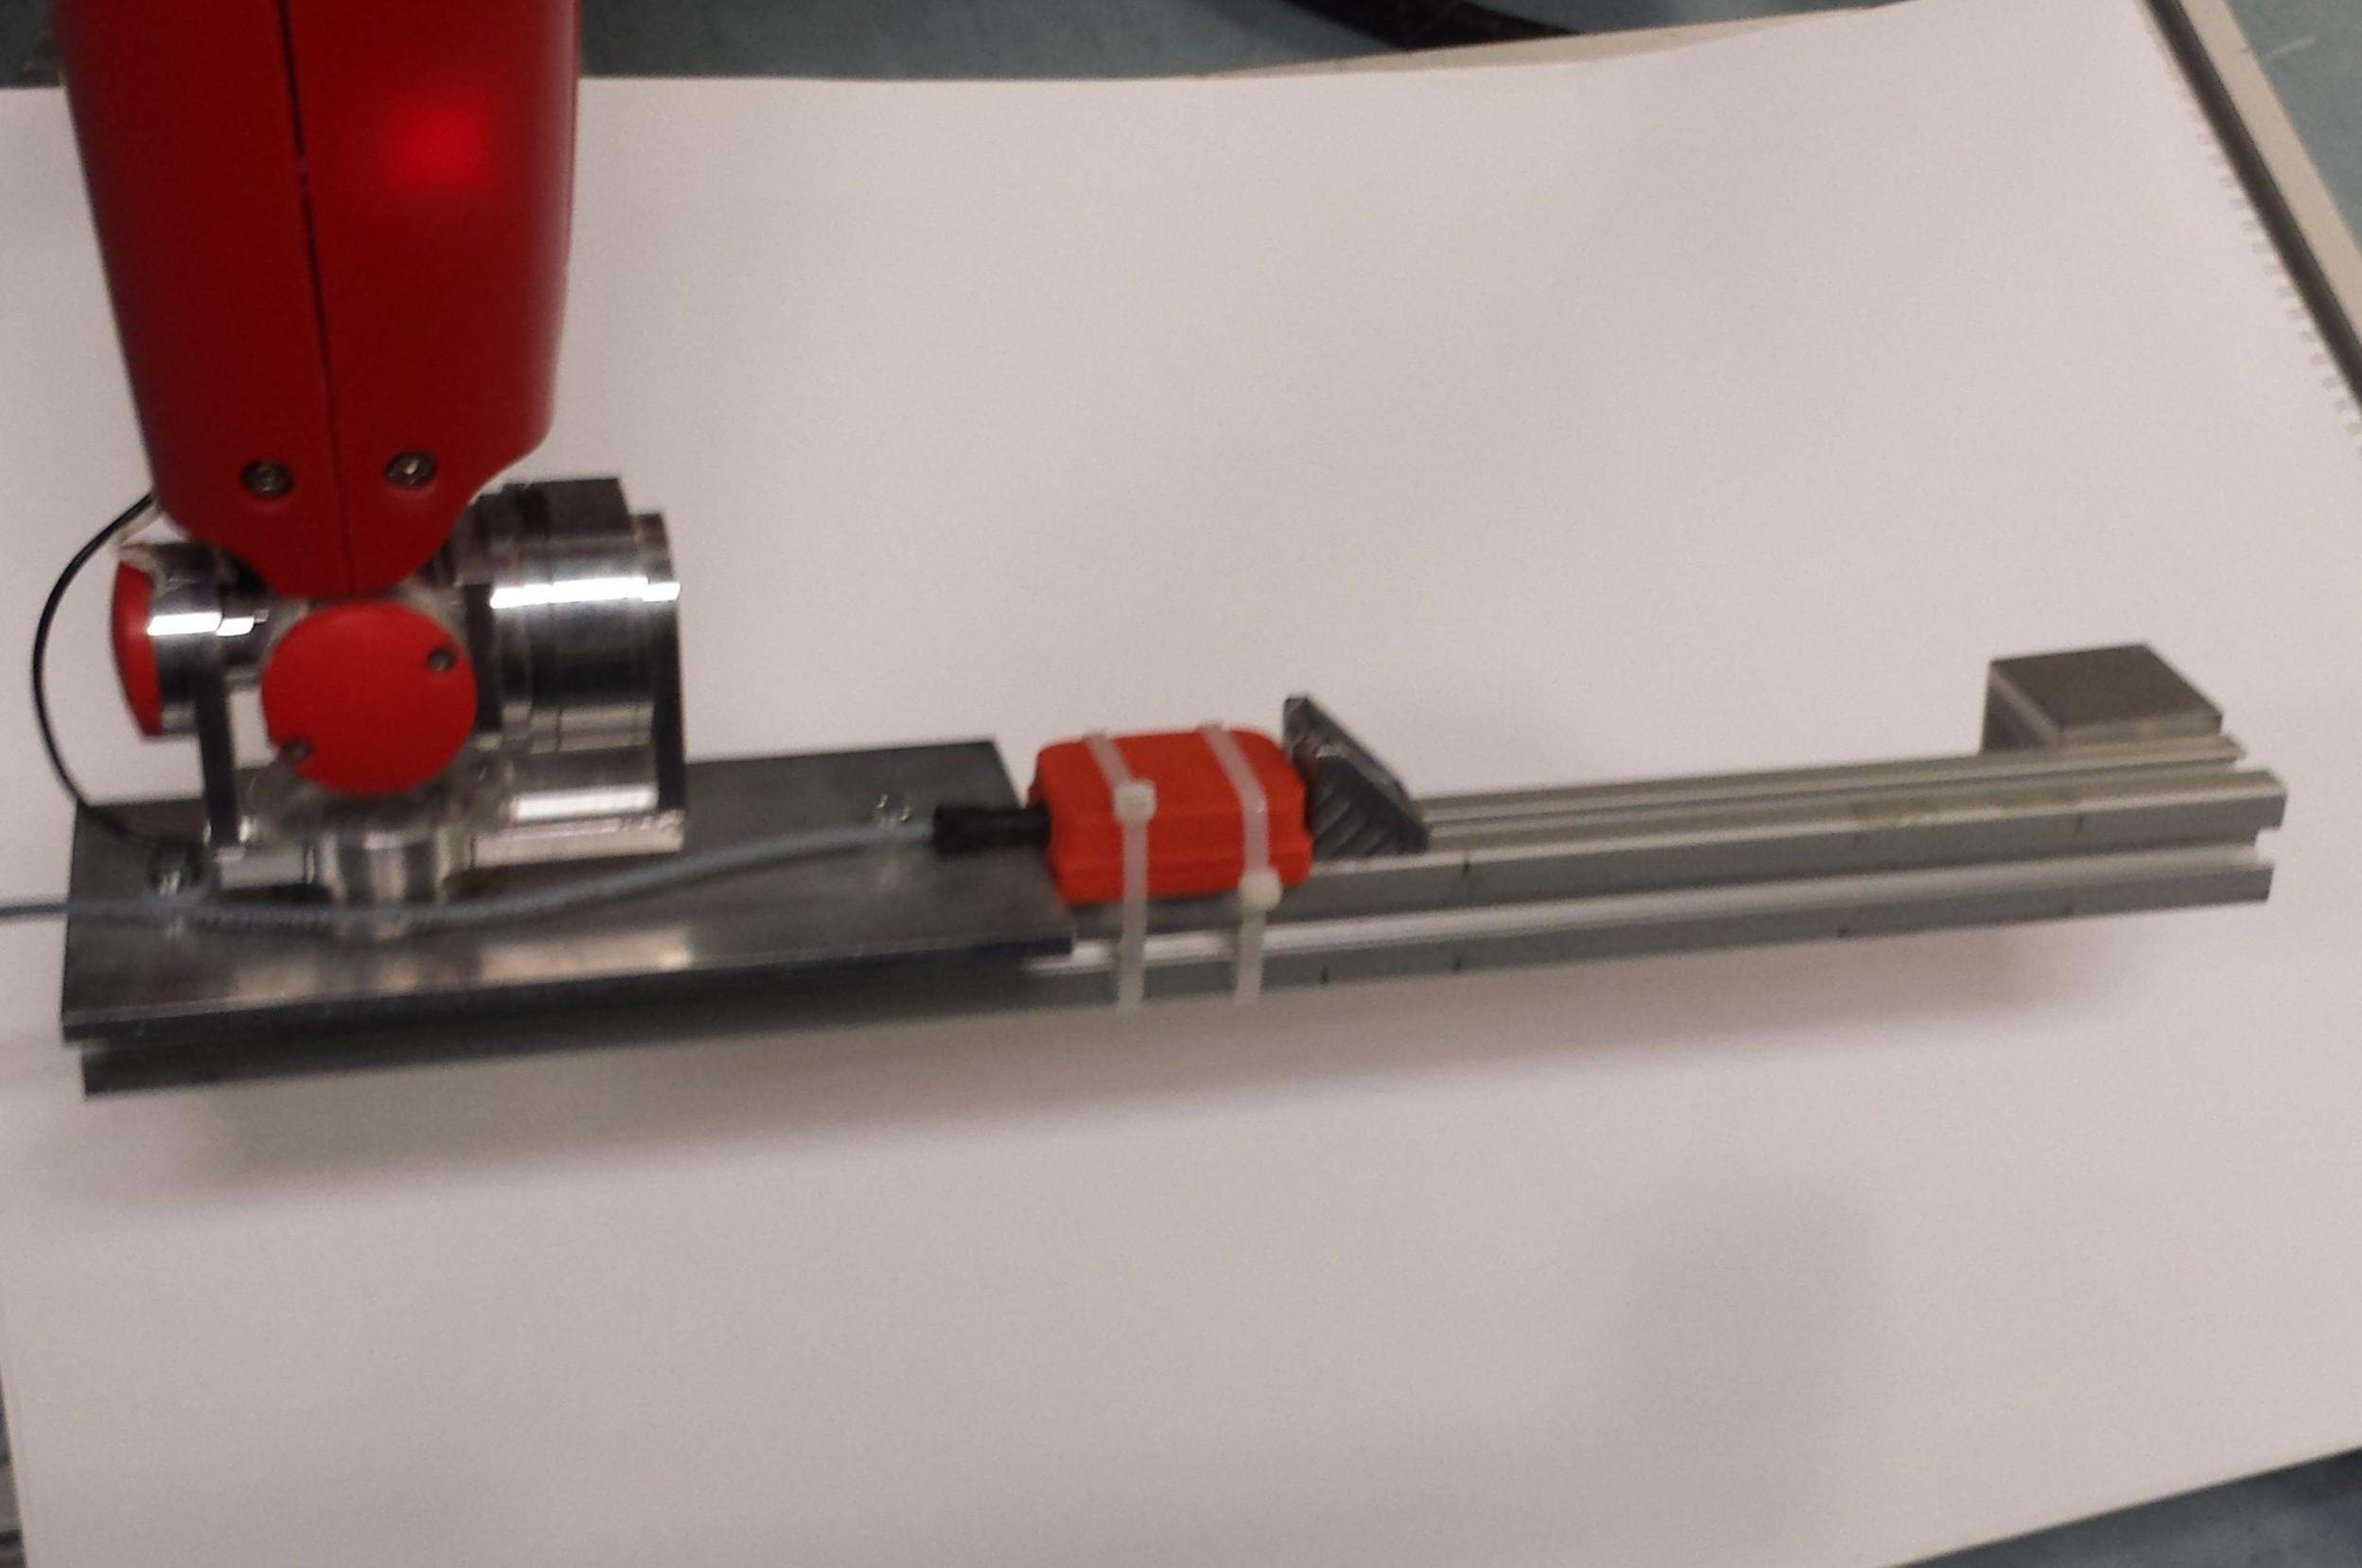
\includegraphics[width=0.48\textwidth]{images/dataset05.pdf}
\label{fig:dataset5}}
\subfloat[Dataset 6]{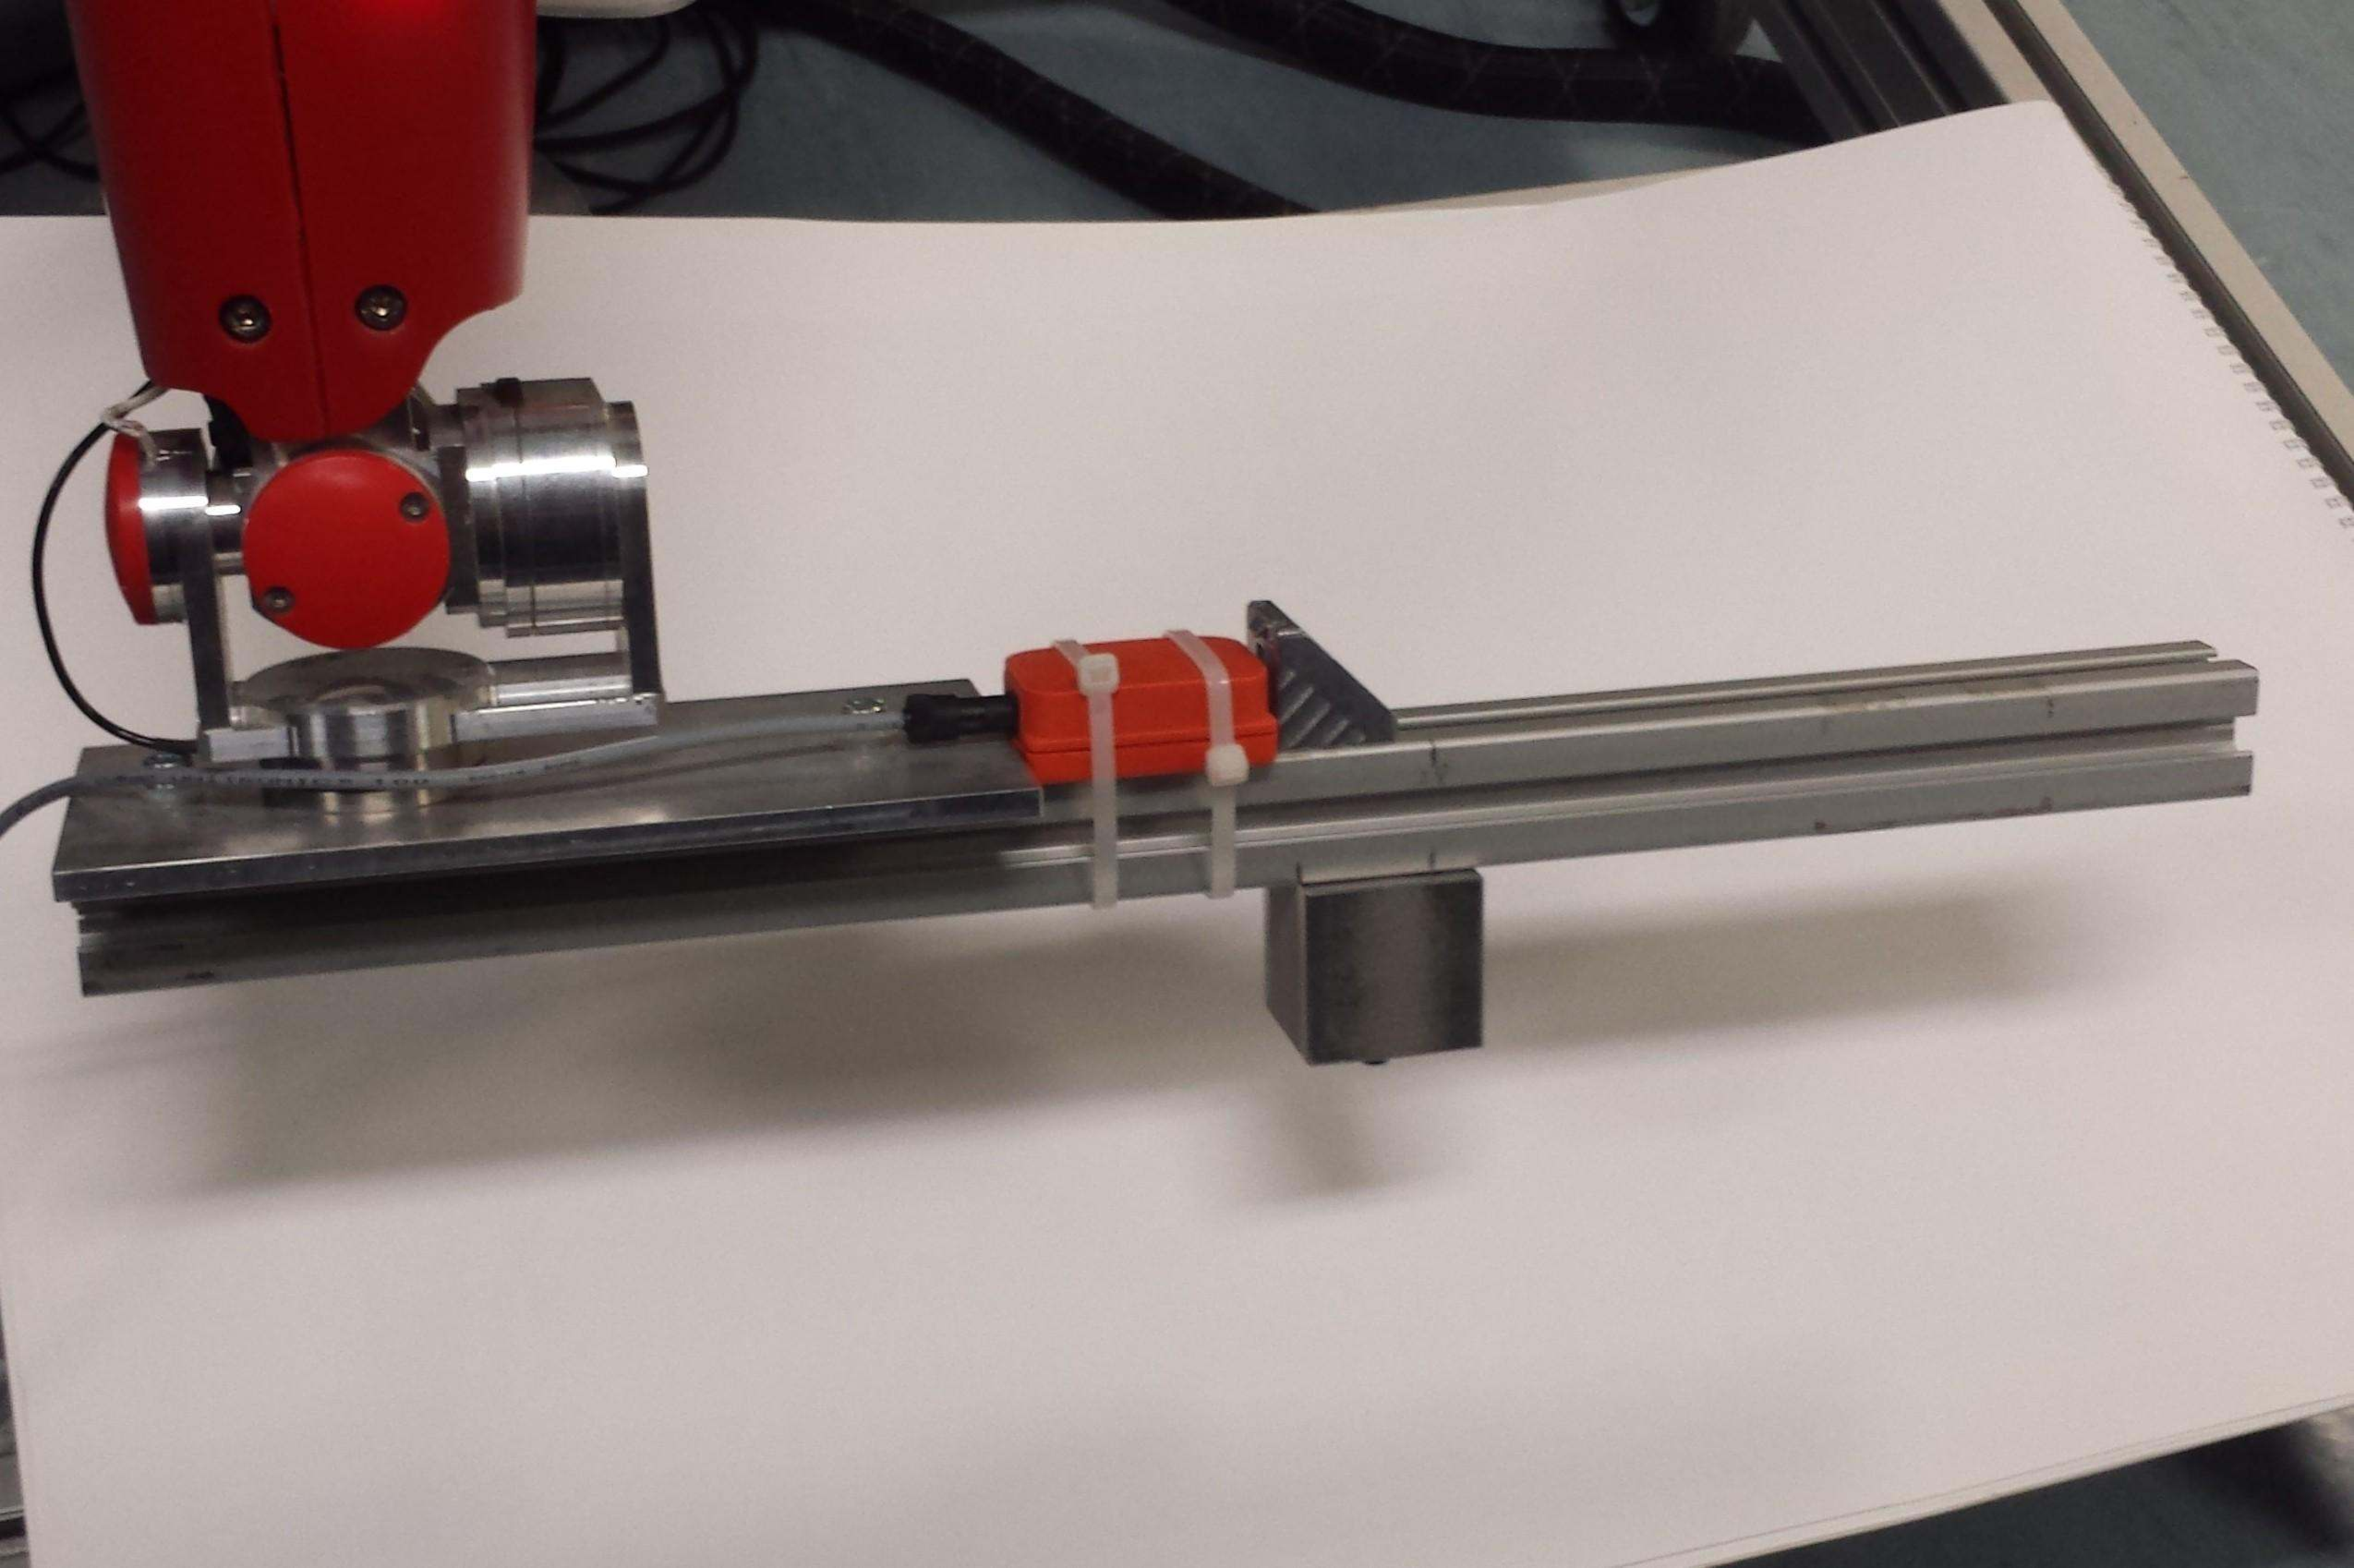
\includegraphics[width=0.48\textwidth]{images/dataset06.pdf}
\label{fig:dataset6}}
 \newline 
\subfloat[Dataset 7: no added mass]{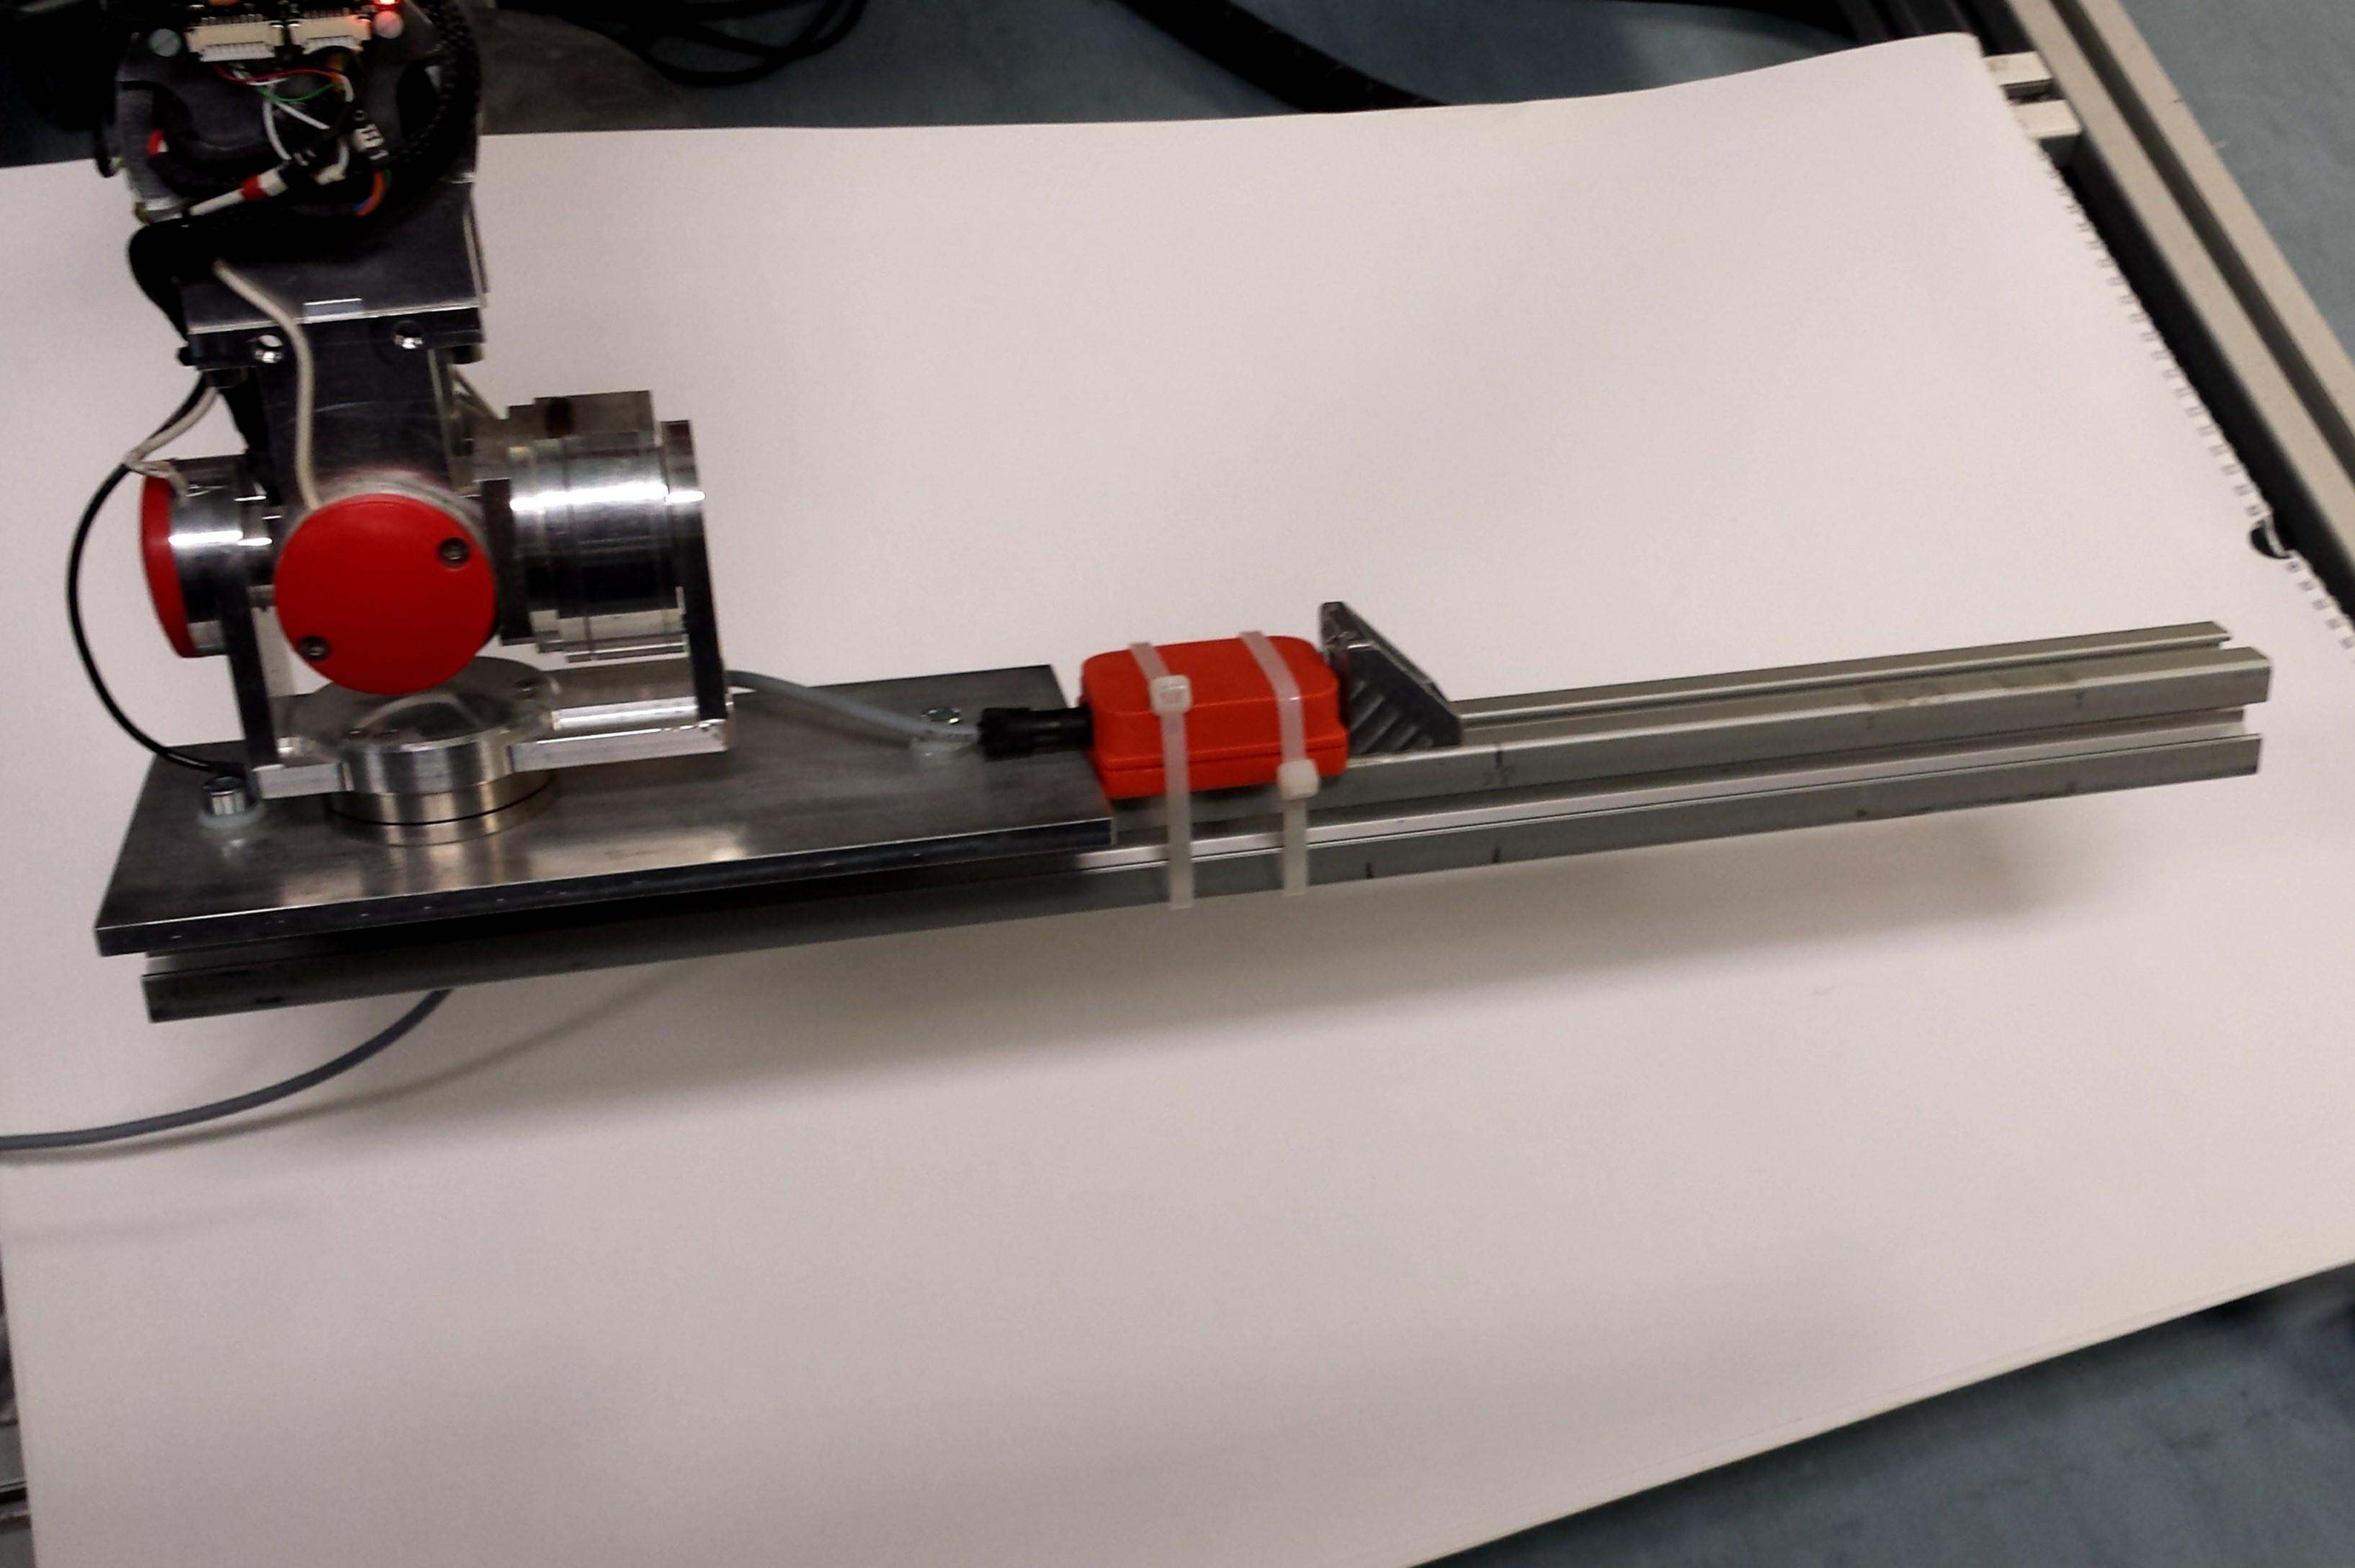
\includegraphics[width=0.48\textwidth]{images/dataset0107.pdf}
\label{fig:dataset7}}
\subfloat[Dataset 8]{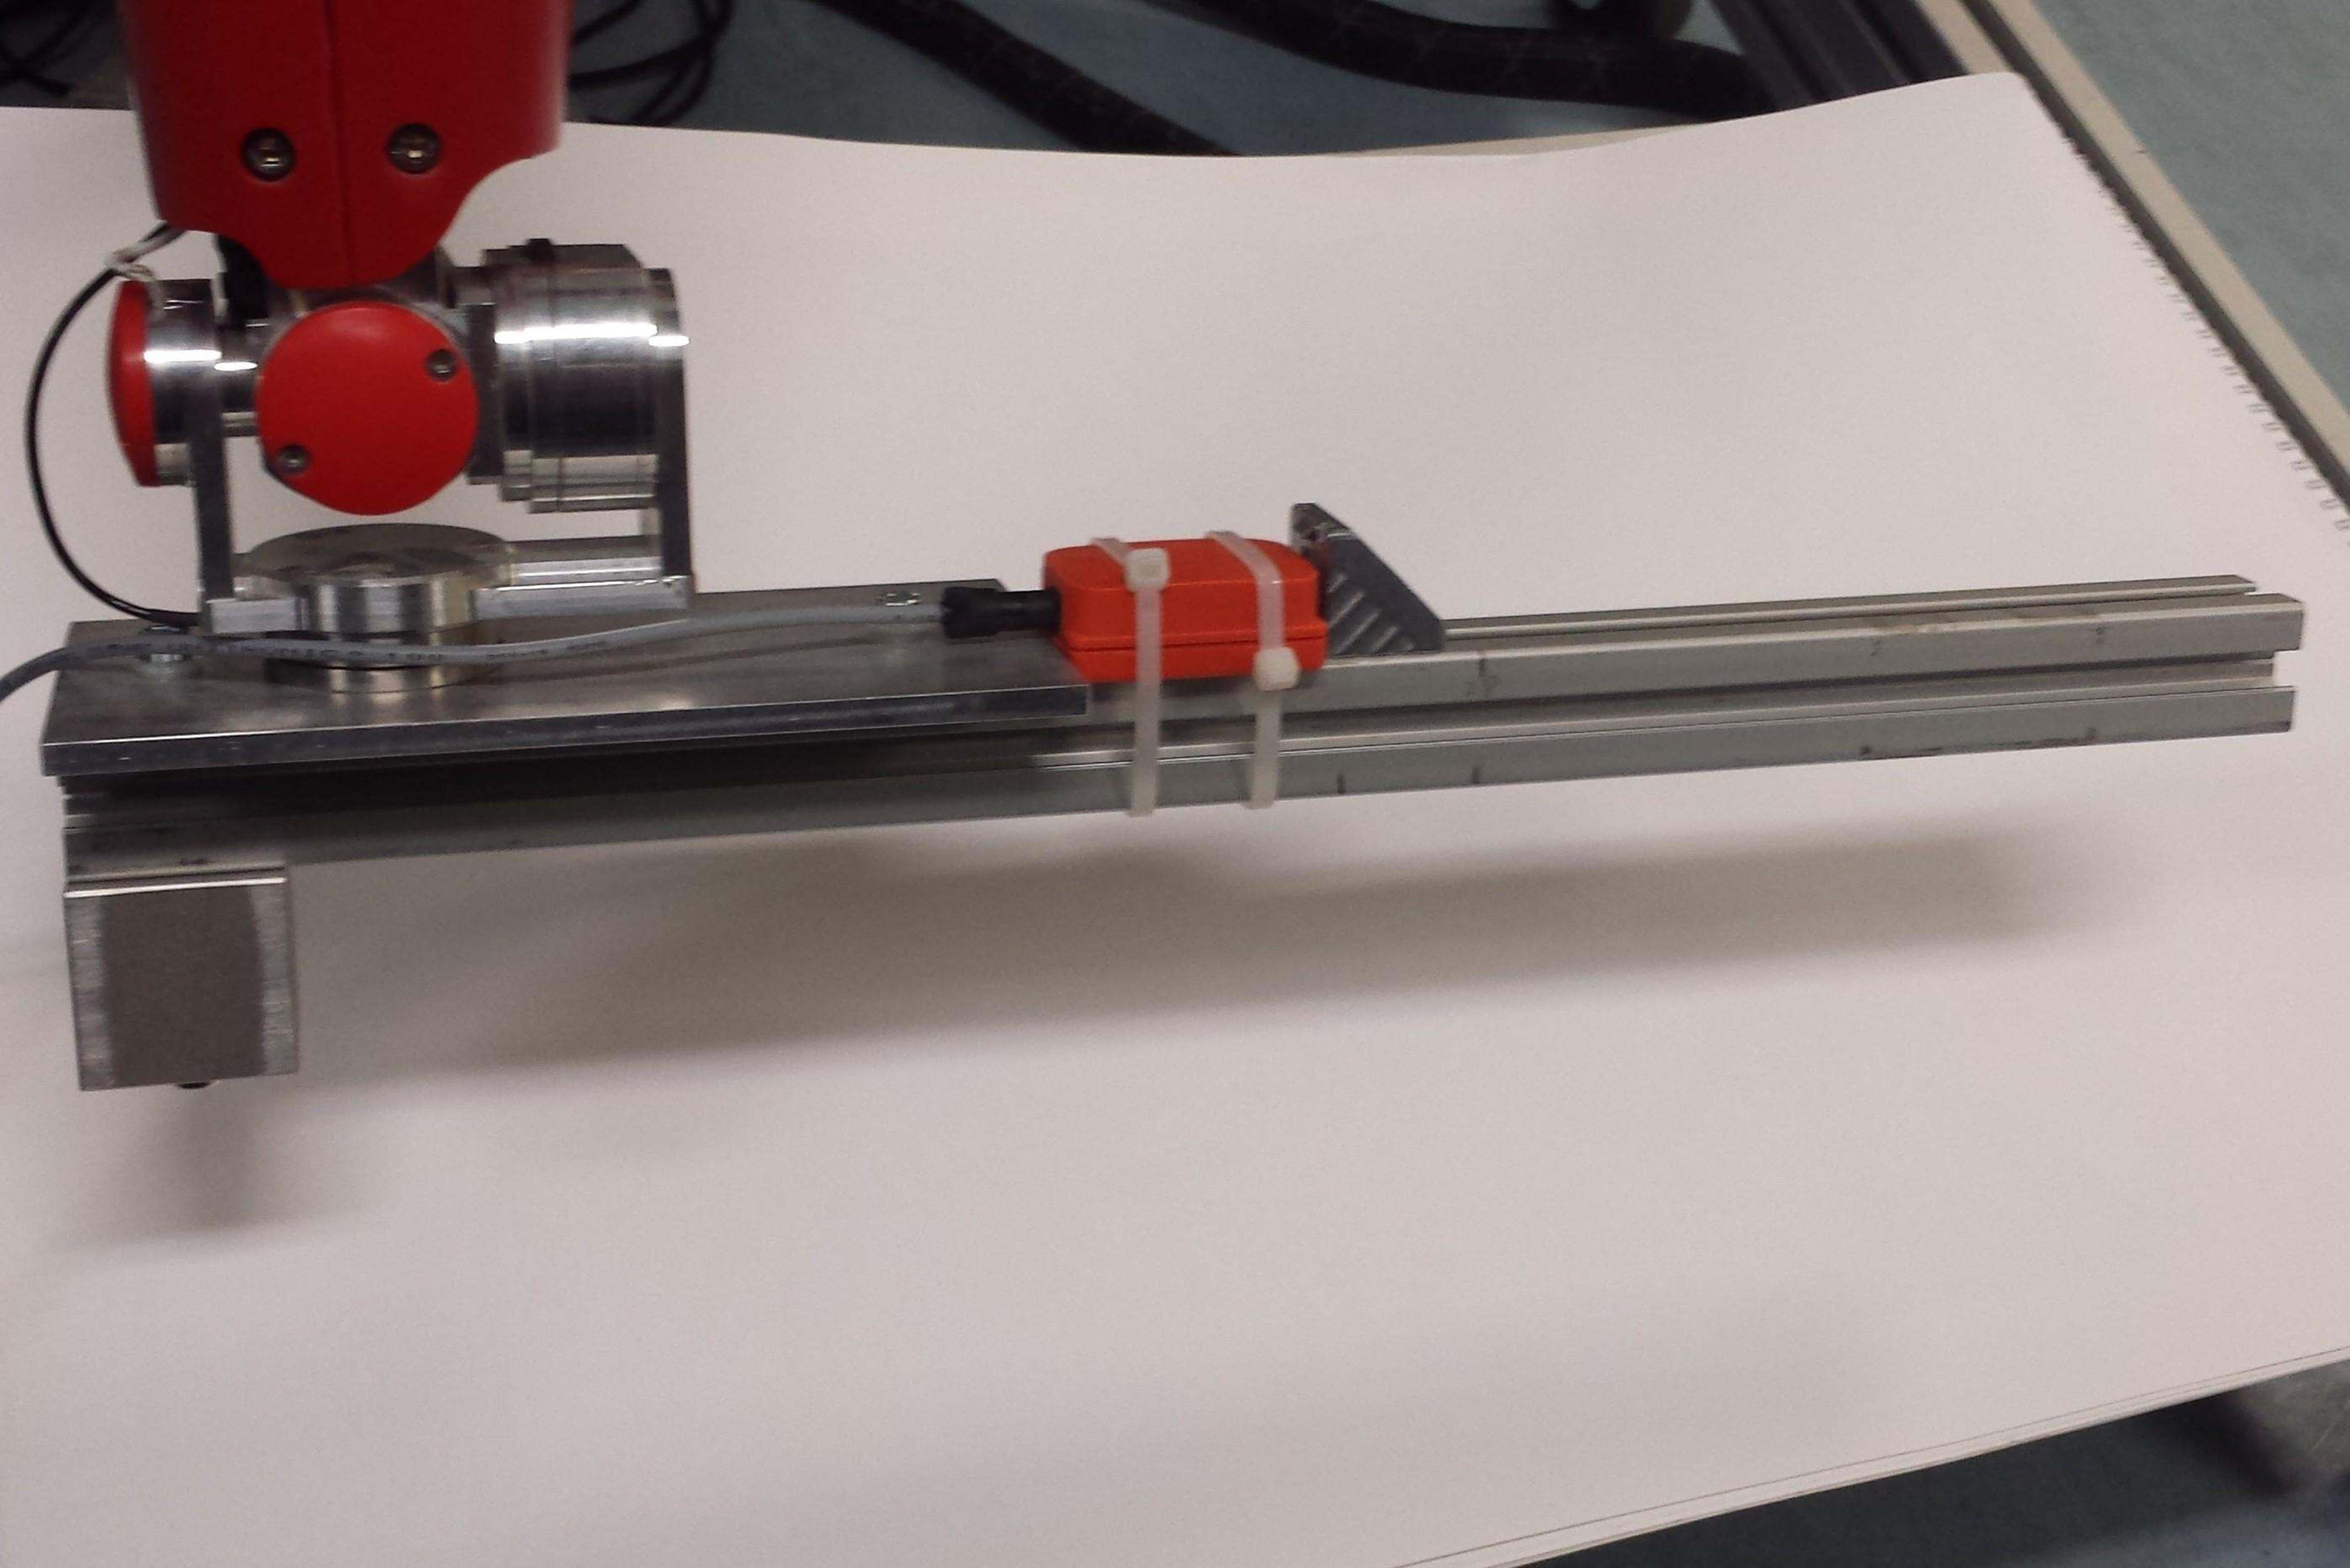
\includegraphics[width=0.48\textwidth]{images/dataset08.pdf}
\label{fig:dataset8}}
\caption{Added mass configurations for validation datasets.}
\label{fig:validation_masses}
\end{figure}


We collected data associated with eight different added mass configurations, each of which is characterized by a mass placed at a different 
location with respect to the beam. In other words, 
we collected eight different data sets. Figures~\ref{fig:calibration} and~\ref{fig:validation_masses} show the configurations of these data sets.

For each of these data sets, we slowly\footnote{The iCub front-back and lateral angles were moved with peak velocities of $2 \deg/s$.} 
moved the \emph{front-back} and
\emph{lateral} angles of the robot hip, spanning a range of $70 \deg$ for the \emph{front-back} angle, and a range of $90 \deg$ for the lateral angle. 
We sampled the two F/T sensors and the accelerometer at 100 Hz, and we filtered the obtained signals with a Savitzky-Golay filter of third order 
with a windows size of 301 samples. 

\begin{figure}
\vspace{0.5em}
 \centering
 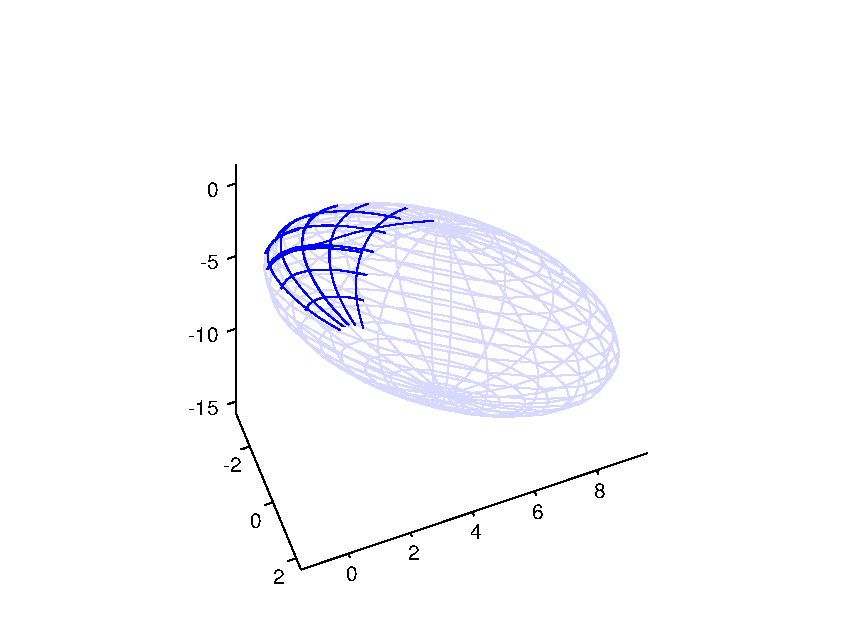
\includegraphics[width=1.0\textwidth]{images/raw_ellipsoid.pdf}
 \caption{Dark blue: raw measurements of the sensor embedded in the leg for dataset 1 projected in the 3D subspace through $U_1$.
 In light blue an ellipsoid fitted to the measured points is added, to highlight the fact that the measured data lie on an ellipsoid. The $o'$ point estimated 
 with the method described in \ref{offsetEstimationTechnique} is the center of this ellipsoid.
  }
 \label{ellipsoidWithRawData}
\end{figure}



We estimated the sensors' offsets by applying the method described in section~\ref{offsetEstimationTechnique} on all eight data sets. 
Figure~\ref{ellipsoidWithRawData} verifies the statement of Lemma~1, i.e. the raw measurements belong to a three dimensional ellipsoid. 
In particular, this figure shows the measurements
$r_i$ projected onto the three dimensional space where the ellipsoid occurs, i.e. the left hand side of the equation~\eqref{rFromModel1}. 
Then, we removed the offset from the raw measurements to apply the estimation method for the calibration matrix described in 
section~\ref{calibrationMatrixEstimation}.

The two sensors' calibration matrices were identified by using only four data sets (see Figure~\ref{fig:calibration}). 
The other four were used to validate the obtained calibration results (see Figure~\ref{fig:validation_masses}).
% Four of these were used for applying the method described in the previous section, and the other
% four for validating this method -- 
The qualitative validation of the calibration procedure is based on the fact that the weight of the leg is constant for each data sets.
Consequently, if we plot
the force measured by the sensors, i.e. the first three rows of left hand side of the sensor's equation
\[ \rmf = C(r - \offset), \]
these forces must belong to a sphere, since they represent the (constant norm) gravity force applied to the sensors.
As for elements of comparisons, we can also plot the first three rows of the above equation when evaluated with the calibration matrix that was 
originally provided by the
manufacturer of the sensors. 

\begin{figure}[ht]
\vspace{0.5em}
\centering
\subfloat[Validation results for leg F/T sensor.]{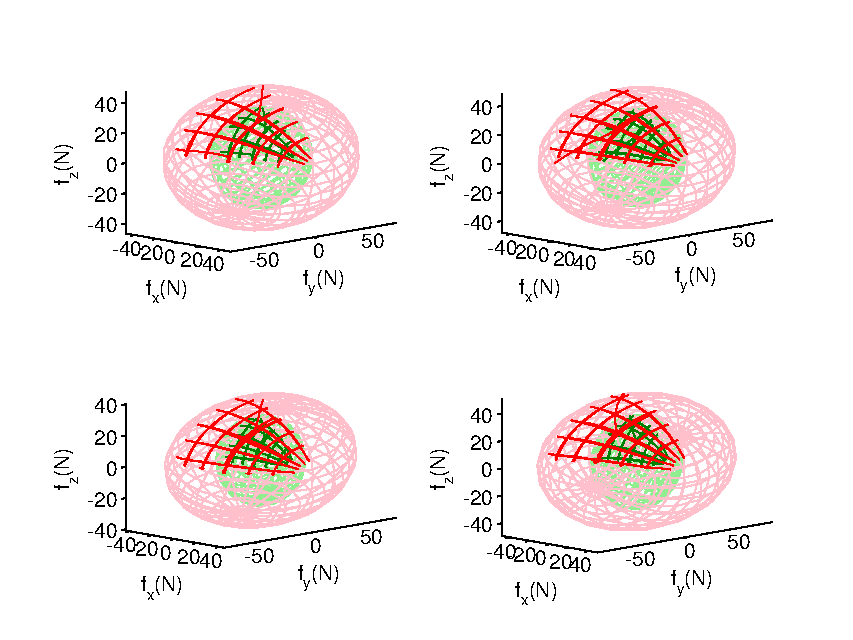
\includegraphics[width=0.8\textwidth]{images/leg_validation.pdf}}
\newline
\subfloat[Validation results for foot F/T sensor.]{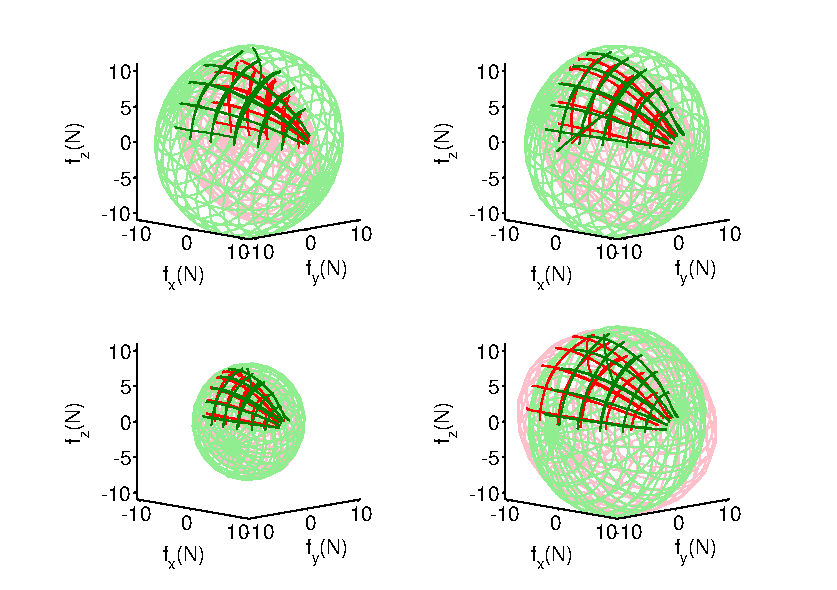
\includegraphics[width=0.8\textwidth]{images/foot_validation.pdf}}
\caption{Dark green: force measurements obtained through the calibration matrix estimated using the proposed technique. Dark red:
force measurements obtained through the calibration matrix provided with the sensor. Light red and light green surfaces: ellipsoids fitted to the 
measured forces.}
\label{fig:validation}
\end{figure}

Figure~\ref{fig:validation} depicts the force measured by the sensor with the estimated calibration matrix (in green)
and with the calibration matrix provided by the manufacturer (in red). It is clear to see that the green surfaces are much more spherical than the red ones.
As a matter of fact, Table \ref{table:soa} lists the semi axes of the ellipsoids plotted in Figures~\ref{fig:validation}, and clearly shows 
that the green surfaces represent spheres much better than the red ones. 
Interestingly enough, the force-torque sensor embedded in the iCub leg is much more mis-calibrated than that embedded in 
the foot. In fact, by looking at the data sheets describing the technological lives of these sensors, we found out that the force-torque sensor embedded in
the leg is much older than that in the foot, which means that the calibration matrix of the leg's sensor is much older than that of the foot's sensor.

%Table \ref{table:mass} shows the quality of the calibration by using the validation dataset for estimating the weight of the sample masses attached to the leg. Both calibrated sensors (at the foot and at the upper leg) are able to give a good estimations of the masses and the improvement with respect to the manufacturer calibration matrix is significant.
%Also in this significant improvement can be seen when using the calibrated matrix as opposed to the original manufacturer calibration.
The quantitative validation of the proposed calibration procedure is performed by comparing the known weights of the added masses with the weights estimated by the sensors. 
Table \ref{table:mass} shows that the estimated weights obtained after performing the proposed calibration are better than those estimated by using the calibration matrix
provided by the sensor manufacturer. A similar comparison was conducted on the estimation of the sample mass positions (Table \ref{table:cmass}). It has to be noticed that the errors in estimating the mass position are relatively high, but this is due to the choice of using relatively small masses with respect to the sensor range and signal to noise ratio.

\begin{table*}[ht] 

\caption{Qualitative calibration evaluation on validation dataset: ellipse semiaxes after calibration}
\centering 
% \begin{tabular}{p{0.8cm} | p{1.2cm} | p{1.2cm}  | p{1.3cm} p{1.3cm} p{1.3cm} | p{1.3cm} p{1.3cm} p{1.3cm}} 
\begin{tabular}{ | c | c | m{1cm} | c c c | c c c | }
\hline
              \emph{Sensor}   & \emph{Dataset} & \emph{Added mass} (Kg) & \multicolumn{3}{p{3.9cm} |}{\emph{Semiaxes length [N] with proposed calibration}} & \multicolumn{3}{p{3.9cm}|}{\emph{Semiaxes length [N] with manufacturer calibration}}\\
\hline \rowcolor[gray]{.9}
  \rowcolor[gray]{.9} Foot    &  5     &  0.51  & 13.6 &  13.1 & 12.9 & 13.5 & 10.2 & 4.6  \\ 
  \rowcolor[gray]{.9} Foot	&  6 & 0.51   & 13.5 & 12.9 & 12.7  & 13.6 & 10.5 & 9.4  \\
  \rowcolor[gray]{.9} Foot	&  7   &  0   & 8.4 & 7.9 & 7.4 & 8.5 &  6.9  & 6.2   \\
  \rowcolor[gray]{.9}  Foot	&  8   &  0.51   & 13.7 & 12.5 & 12.0 & 15.7 & 13.6 & 10.4  \\
 \hline 
 Leg  &  5    & 0.51   & 34.4 & 33.3 & 32.5 & 76.5 & 49.4 & 45.6 \\ 
 Leg	&  6  & 0.51  & 34.8 & 33.5 & 32.8  & 82.4 & 49.3 & 47.3  \\
 Leg	&  7  & 0     & 30.9 & 28.2 & 26.9   & 77.0 & 44.5  & 40.0 \\
 Leg	&  8  & 0.51   & 35.52 & 33.30 & 32.2 & 88.9 & 49.5 & 48.3   \\
\hline

\end{tabular} 
\label{table:soa} %\bigskip
\end{table*}

\begin{table*}[ht] 
\caption{Qualitative calibration evaluation on validation dataset: sample mass estimations}
\centering 
% \begin{tabular}{p{0.8cm} | p{1.3cm} | p{2cm}  | p{2cm} | p{2cm} } 
\begin{tabular}{ | c | c | c | c | c | } 
\hline
              \emph{Sensor}   & \emph{Dataset} & \multicolumn{3}{c|}{\emph{Added mass} (Kg)} \\
\hline \rowcolor[gray]{.9}
\hline \rowcolor[gray]{.9}    &                &  \multicolumn{1}{p{1.6cm}|}{Ground truth} & \multicolumn{1}{p{2cm}|}{Proposed calibration} & \multicolumn{1}{p{2.2cm}|}{Manufacturer calibration}     \\
\hline
  \rowcolor[gray]{.9} Foot    &  5     &  0.51    &  0.53  & 0.06  \\ 
  \rowcolor[gray]{.9} Foot	&  6   &  0.51    &  0.52   &  0.27  \\
  \rowcolor[gray]{.9} Foot	&  7   &  0       & -0.03  &  -0.13 \\
  \rowcolor[gray]{.9}  Foot	&  8   &  0.51    &  0.46  & 0.45 \\
 \hline 
 Leg  &  5    & 0.51  & 0.51 & 2.77  \\ 
 Leg	&  6  & 0.51  & 0.54 & 3.04  \\
 Leg	&  7  & 0     & -0.04  & 2.39  \\
 Leg	&  8  & 0.51  & 0.51  & 3.25  \\
 \hline
 \end{tabular} 
 \label{table:mass} %\bigskip
 \end{table*}

 \begin{table*}[ht] 
 \caption{Qualitative calibration evaluation on validation dataset: center of mass estimations}
 \centering 
 % \begin{tabular}{p{1.4cm} | p{2.2cm} | p{1.4cm} |  p{0.7cm} |  p{0.7cm}  ||  p{0.7cm} |  p{0.7cm} |  p{0.7cm}||  p{0.7cm} |  p{0.7cm} |  p{1.2cm} } 
  \begin{tabular}{ | c | c | c |  c |  c | c | c |  c | c |  c | c |} 
  \hline
              \emph{Sensor}   & \emph{Dataset} & \multicolumn{9}{c|}{\emph{Center of mass position for the added mass} [cm]} \\
 \hline \rowcolor[gray]{.9}   &             &  \multicolumn{3}{c|}{Ground truth} &  \multicolumn{3}{p{2.8cm}|}{Proposed \hspace{3em}  calibration} & \multicolumn{3}{p{3cm}|}{Manufacturer calibration} \\ 
 \hline
  \rowcolor[gray]{.9} Foot    &  5     & 39  & {-}3.5 & 2.9  & 31  & 8.8 & $-$8.3  & 273  & $-$83 & 81  \\ 
  \rowcolor[gray]{.9} Foot	&   6   &  21 &  0   & 6.3  & 19  & 9.9 & $-$5    & 30   & $-$18 & 18  \\
  \rowcolor[gray]{.9} Foot	&  7   &  -  & -    & -    & -   &  -  & -     & -    &  -  & -  \\
  \rowcolor[gray]{.9}  Foot	&  8   &  {-}4 & 0   & 6.3  & 5.5 &  9  & $-$3.2  & $-$8.6 & $-$12 & 10 \\
 \hline 
 Leg  &  5    & 39 & $-$3.5 & 39  & 28 & 11 & 29 & 16 & 6.5 & 29  \\ 
Leg	&  6  & 20 & 0  & 43  & 17 & 9.7 & 30 & 12 & 5.1 & $-$27  \\
Leg	&  7  & -  & -  & -   & -  & -   & -  & -  & -   & -  \\
 Leg	&  8  & $-$4.3 & 0 & 43 & 3.8 & 8.8 & 32 & 7.5 & 4.9 & $-$26 \\
\hline
\end{tabular} 
\label{table:cmass} %\bigskip
\end{table*}


% Figures~\ref{fotoPesi}~\ref{fotoPesi}.  


